\documentclass[a4paper,oneside]{ltjsarticle}
\usepackage{amsmath}
\usepackage{tikz}
\usetikzlibrary{positioning,arrows,shapes,chains}
\usepackage{listings}
\lstset{
	float=hbp,
	basicstyle=\ttfamily,
	numberstyle=\ttfamily\footnotesize,
	identifierstyle=,
	columns=flexible,
	tabsize=2,
	frame=single,
	extendedchars=true,
	inputencoding=utf8x,
	showspaces=false,
	showstringspaces=false,
	numbers=left,
	breaklines=true,
	breakautoindent=true,
	captionpos=t,
}
\title{AT-TaPL 4: Typed Assembly Language pt.1}
\author{河原 悟}
\begin{document}
\maketitle
P142〜

\setcounter{section}{-1}
\section{introduction}
適当に引っ張ってきたコードは正しく動くのか?
\begin{itemize}
	\item \textit{proof-carrying code(PCC)} by Necula amd Lee

		コードの性質の証明のチェックが簡単できて、proof-checking engineが小さい
\end{itemize}

PCCをうまく使っていくために、以下の問題を解決したい:

\begin{enumerate}
	\item コードが満たすべき性質とは?
	\item コードが満たすべき性質の証明をプログラマーはどう作るか?
\end{enumerate}

1. は文脈やアプリケーションに依存し、2. は自動的にはできない。ではどうするか?

\textit{type-preserving} compilationをベースにしたアプローチを考えてみる。
コードが満たすべき性質として型安全であることにフォーカスする。

この方法論では、コンパイルのプロセスとして型付きマシンコードにコンパイルされる型付きの中間言語をデザインする必要がある。
\begin{figure}[h]
	\centering
	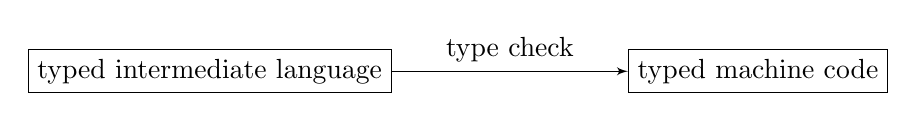
\begin{tikzpicture}
		\node[draw] (A) {typed intermediate language};
		\node[right = 3 of A,draw] (B) {typed machine code};
		\path[draw,-latex'] (A) -- node[midway,above] { type check }  (B);
	\end{tikzpicture}
	\caption{必要となる工程}
\end{figure}

CISCライクではなく、RISCライクな、高級言語の機能をエンコードでき種々の最適化が適用できる言語を考える。

\section{TAL-0: Control-Flow-Safety}
まずRISCスタイルの型付きアセンブリー言語を考えるにあたり、\textit{control-flow safety}という性質にフォーカスしてみる。
直感として、意図しないアドレスへのジャンプを防ぎ、適切なエントリーポイントにのみ飛ぶことができるように制御する。

\newpage
\begin{figure}[ht]
	\noindent\hrulefill

	\begin{minipage}[h]{.48\textwidth}
		\begin{align*}
			&r\ \mathtt{::=}&&&registers:&\\
			 &&&\mathtt{r1\ \mid\ r2\ \mid\ \cdots\ \mid\ rk}&&&\\
			 &v\ \mathtt{::=}&&&operands:&\\
			 &&n&&integer\ literal&\\
			 &&l&&label\ or\ pointer&\\
			 &&r&&registers&
		\end{align*}
	\end{minipage}\hfill
	\begin{minipage}[h]{.02\textwidth}
		\begin{center}
			\begin{tikzpicture}
				\coordinate (A) at (0, 0);
				\coordinate (B) at (0, -4);
				\draw[-] (A) -- (B);
			\end{tikzpicture}
		\end{center}
	\end{minipage}
	\begin{minipage}[h]{.48\textwidth}
		\hfill\begin{align*}
			&i\ \mathtt{::=}&&&instructions:&\\
			 &&&r_d\mathtt{:=}v&&&\\
			 &&&r_d\mathtt{:=}r_s\mathtt{+}v&&&\\
			 &&&\mathtt{if}\ r\ \mathtt{jump}\ v&&&\\
			 &I\ \mathtt{::=}&&&instruction\ sequences:&\\
			 &&&\mathtt{jump}\ v&&&\\
			 &&&i;I&&&
		\end{align*}
	\end{minipage}

	\noindent\hrulefill
	\caption{Instructions and operands for TAL-0}
\end{figure}

\begin{figure}[ht]
	\noindent\hrulefill

	\begin{minipage}[h]{.48\textwidth}
		\begin{align*}
			&R\ \mathtt{::=}&&&register\ files:&\\
			&&&\{\mathtt{r_1\ =\ }v_1,\dots ,\mathtt{r_k\ =\ }v_k\}&&&\\
			&h\ \mathtt{::=}&&&heap\ values:&\\
			&&I&&code&
		\end{align*}
	\end{minipage}\hfill%
	% \begin{minipage}[h]{.02\textwidth}
		% \begin{center}
			% \begin{tikzpicture}
				% \coordinate (A) at (0, 0);
				% \coordinate (B) at (0, -1);
				% \draw[-] (A) -- (B);
			% \end{tikzpicture}
		% \end{center}
	% \end{minipage}
	\begin{minipage}[h]{.48\textwidth}
		\hfill\begin{align*}
			&H\ \mathtt{::=}&&&heaps:&\\
			&&&\{l_1\ =\ v_1,\dots ,l_k\ =\ v_k\}&&&\\
			&M\ \mathtt{::=}&&&&machine\ states:&\\
			% &&&\(H,R,I\)&&&
		\end{align*}
	\end{minipage}

	\noindent\hrulefill
\end{figure}

\texttt{mov}や\texttt{add}のような表記よりfamiliarな表記を用いる。

\begin{lstlisting}
prod: r3 := 0;
    jump loop

loop: if r1 jump done;
    r3 := r2 + r3;
    r1 := r1 + -1;
    jump loop

done: jump r4
\end{lstlisting}
\end{document}

